% !TEX TS-program = xelatex

\documentclass{beamer}
\usetheme{default}

\usepackage{ctex}

\title{Rumor Diffusion Model Based on Representation Learning and Anti-Rumor}
\author{张展鹏}
\begin{document}
\begin{frame}[plain]
    \maketitle
\end{frame}

\begin{frame}{关于谣言扩散模型,我们应该知道的……}
	\begin{itemize}
		\item RUMOR refers to information and statements that have not been officially confirmed and are inconsistent with facts.
		\item 新冠疫情导致了大量谣言在网络扩散,造谣、传谣、辟谣,谣言传播相关研究是时下热点。
		\item Online rumors can quickly spread their influence and can even spread faster and more widely than real information because of their concealment, suddenness, and dispersion (隐蔽性、突然性和分散性)。
	\end{itemize}
\end{frame}

\begin{frame}{当前研究方法 vs 论文研究方法}
	\begin{itemize}
		\item 当前研究方法:传染病模型和机器学习
		\begin{itemize}
			\item 传染病模型是一种描述性的方法。类比传染病网络中存在超级传染者、携带者、易感者和不易感者等,对谣言传播网络中存在的节点进行分类。
			\item 机器学习从数据集出发,学习机器学习的传播特点。
		\end{itemize}
		\item 论文研究方法:特征学习+博弈论
		\begin{itemize}
			\item 特征学习,输入用户发布历史和社交网络,获得用户向量;考虑了信息空间多样性,运用了多种学习方法。
			\item 博弈论,谣言(rumor)和辟谣(anti-rumor)是共生和竞争的,博弈论和多元线性回归是用来描述谣言传播的拓扑特征的。
		\end{itemize}
		\item 论文应用了谣言和辟谣的动态传播模型和CNN-GCN解决了输入数据不平衡问题。论文的亮点之一是真实地模拟了谣言扩散——谣言传播空间的非欧特征;谣言的生命周期。
	\end{itemize}
\end{frame}

\begin{frame}{谣言扩散场景例子}
	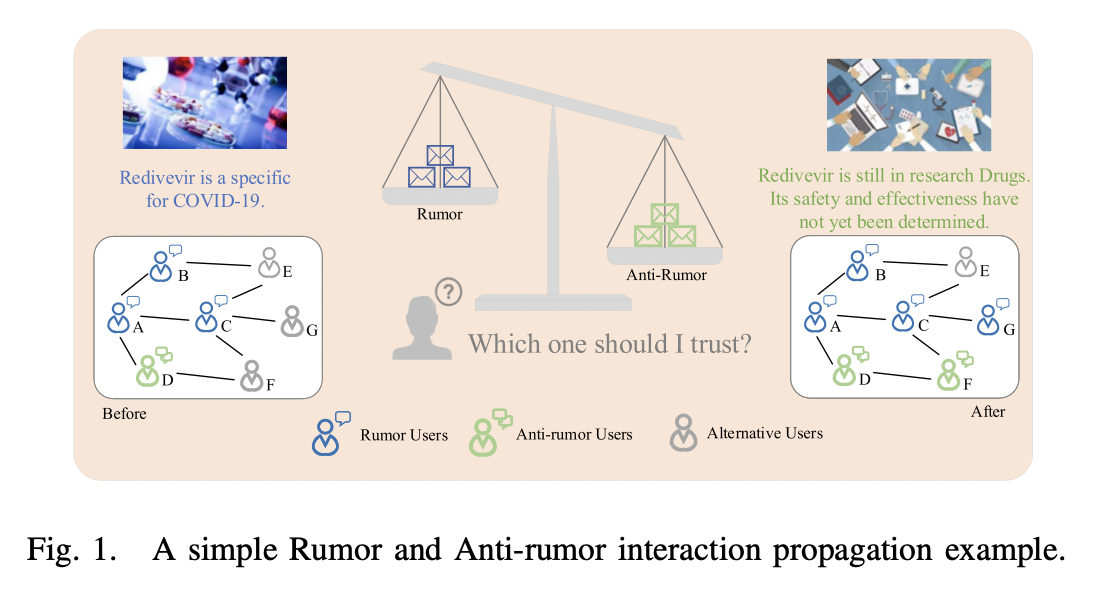
\includegraphics[width=\linewidth]{Assets/图1}
\end{frame}

\begin{frame}{论文相关工作(1)——转发行为预测}
	谣言话题复杂,属性多,数据维度高。研究入手角度一般是用户的个人信息和行为特征。
	\begin{itemize}
		\item 用户的转发行为会影响朋友,预测用户的转发行为。
		\item 用户转发内容的倾向收到一系列因素影响,挖掘影响因素。
	\end{itemize}
	上述研究注重从社交网络中提取特征,对社交网络缺乏合理表示,未考虑非欧几里得结构,即超图特征。事实上,社交网络是一个典型的小世界网络,仅用节点和边很难真实描述真实世界,它存在一些超边。
\end{frame}

\begin{frame}{论文相关工作(2)——谣言和辟谣,话题多样性}
	学者们建立了多种谣言传播模型,描述谣言传播中节点的变化。同时,学者们也考虑了其他消息对谣言传播的影响,即辟谣对谣言的抑制作用。
	\begin{itemize}
		\item 谣言传播类似传染病流行,考虑了节点活动的影响,例如节点流动性、节点角色变化、节点识别能力差异等。
		\item 正面新闻常常跟负面新闻同时传播,这可以类比成传染病的免疫机制,正面新闻对负面新闻有抑制作用。
	\end{itemize}
	上述研究虽然考虑了辟谣跟谣言共同传播的情形,但是不够完整。辟谣和谣言的关系是共生和竞争的,存在更深刻的相互作用,仅考虑辟谣对谣言的抑制是不够的。
\end{frame}

\begin{frame}{论文相关工作(3)——特征学习和博弈论}
	\begin{itemize}
		\item 特征学习可以来减轻数据稀疏性带来的不利影响。
		\item 博弈论可以用来研究社交网络中用户之间的互动,预测个人行为。
	\end{itemize}
\end{frame}

\begin{frame}{相关研究面临的挑战}
	\begin{itemize}
		\item 谣言传播借助社交网络进行,用户之间的社交和利益关系是研究谣言传播的基础,论文需要良好地结合社交网络的拓扑特征。
		\item 在现实生活中,公共媒体的辟谣作用不能忽视,辟谣会减缓谣言传播;减缓效应难以量化。
		\item 数据集规模小,这意味着谣言和辟谣数据不平衡。
	\end{itemize}
\end{frame}

\begin{frame}{论文研究目标}
	\begin{itemize}
		\item Predict whether potential users in the rumor topic will forward the rumor message or forward the anti-rumor message.
		\item Predict the development trend of rumor topics.
	\end{itemize}
	论文的核心任务是预测用户对谣言和辟谣的转发行为。
\end{frame}

\begin{frame}{用户 = 造/传谣者 + 辟谣者 + 潜在用户}
	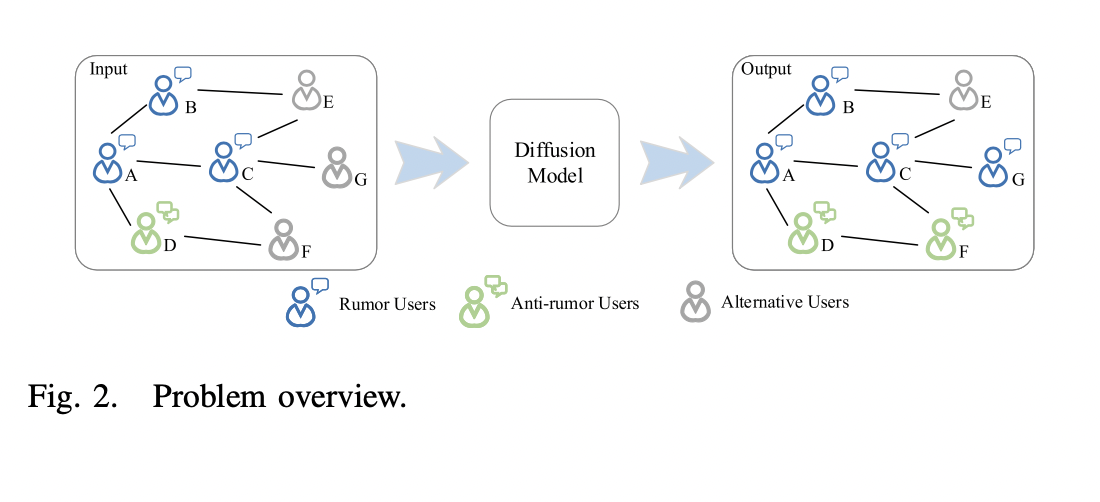
\includegraphics[width=\linewidth]{Assets/图2}
	Alternative users = Rumor potential users + Anti-rumor potential users
\end{frame}

\begin{frame}{用户属性 = 活跃度 + 表达方式偏好 + 社交影响力}
	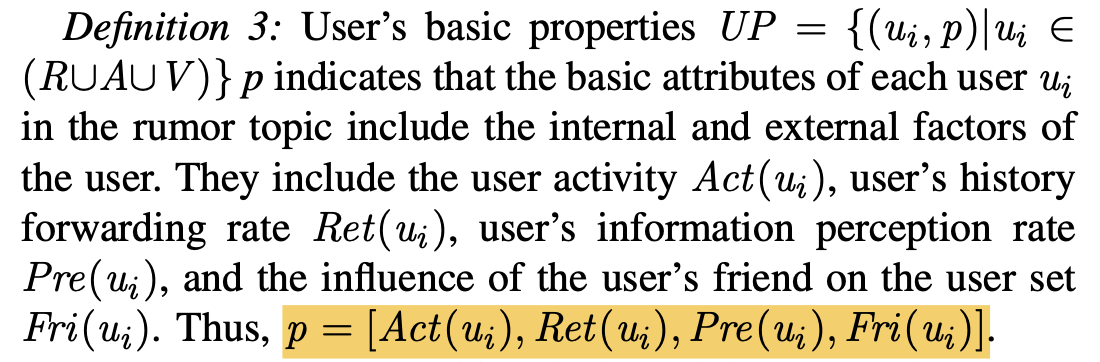
\includegraphics[width=\linewidth]{Assets/定义3.png}
	用户属性描述了活跃度、表达个人看法和转发倾向以及他/她对朋友的影响力。
\end{frame}

\begin{frame}{用户历史内容 -> 一篇分段的文章}
	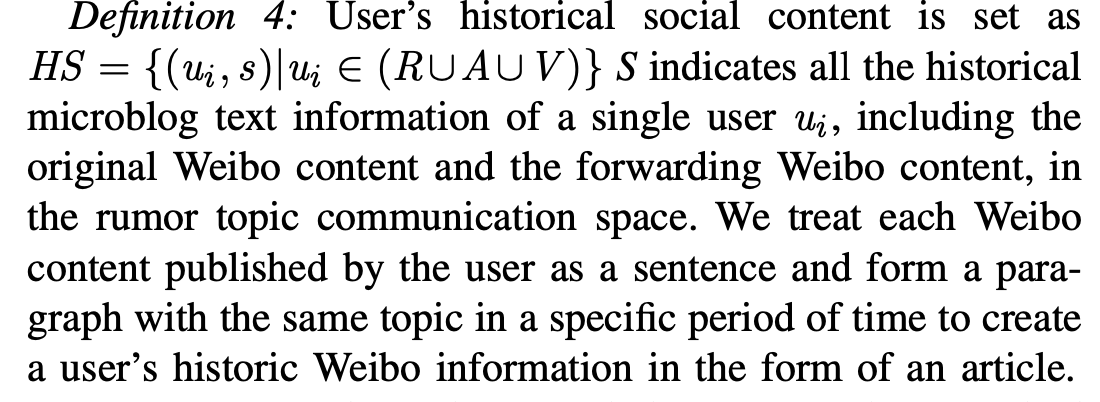
\includegraphics[width=\linewidth]{Assets/定义4.png}
	用户历史内容被处理成一篇格式整齐的文章。
\end{frame}

\begin{frame}{谣言流行度存在半衰期}
	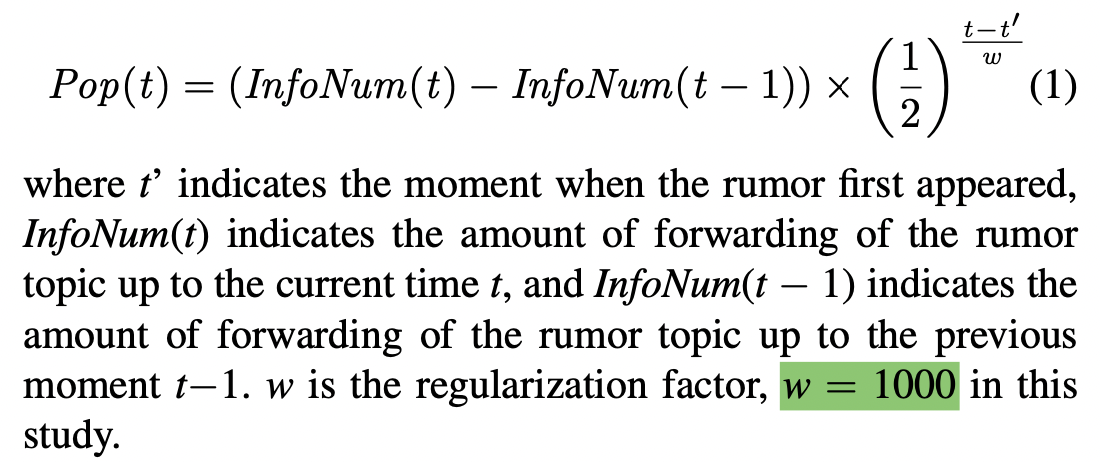
\includegraphics[width=\linewidth]{Assets/定义5.png}
	流行度通过被转发数目量化。谣言总是突然出现并快速到达流行度峰值,随着对应的辟谣信息出现,它的流行度会随时间半衰。这个规律已经在文献中被报道。
\end{frame}

\begin{frame}{用数学语言描述待解决的问题}
	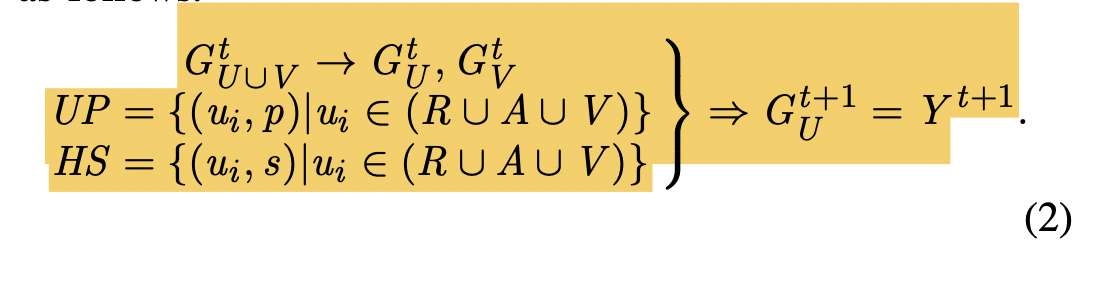
\includegraphics[width=\linewidth]{Assets/公式2.png}
	输入:
	\begin{itemize}
		\item 社交网络中已经接触谣言/辟谣信息的用户子图和其他用户,即潜在用户子图
		\item 每个用户的属性
		\item 每个用户的历史内容
	\end{itemize}
	输出:
	\begin{itemize}
		\item 下一时间,社交网络中已经接触谣言/辟谣信息的用户子图,新用户是相信并传播谣言还是参与辟谣。
	\end{itemize}
\end{frame}

\begin{frame}{解决问题的总方法}
	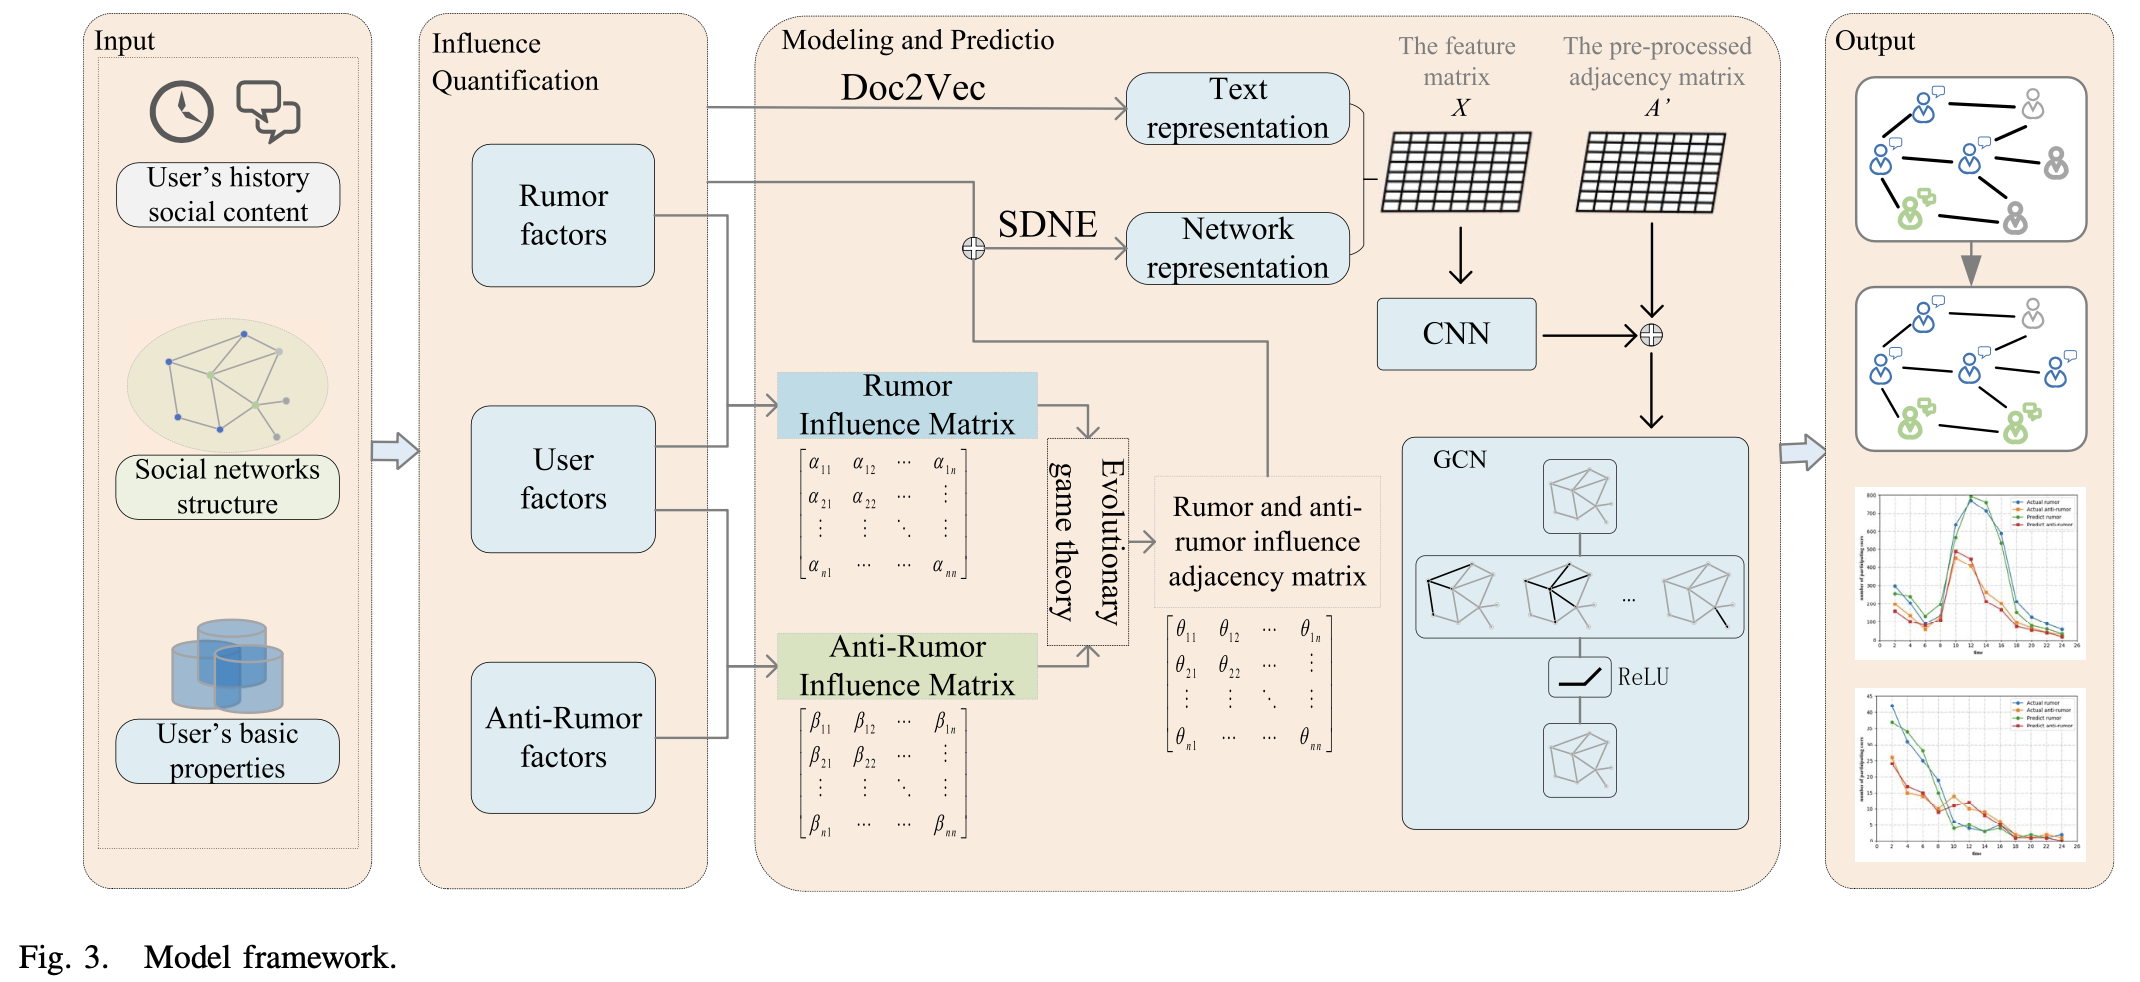
\includegraphics[width=\linewidth]{Assets/图3.png}
\end{frame}

\begin{frame}{谣言主题特征的表示}
	论文应用了SDNE(Structural Deep Network Embedding ),一种用来进行网络表示学习的方法。SDNE同时优化一阶和二阶相似度,能够保留局部和全局结构,对稀疏网络具有鲁棒性。
	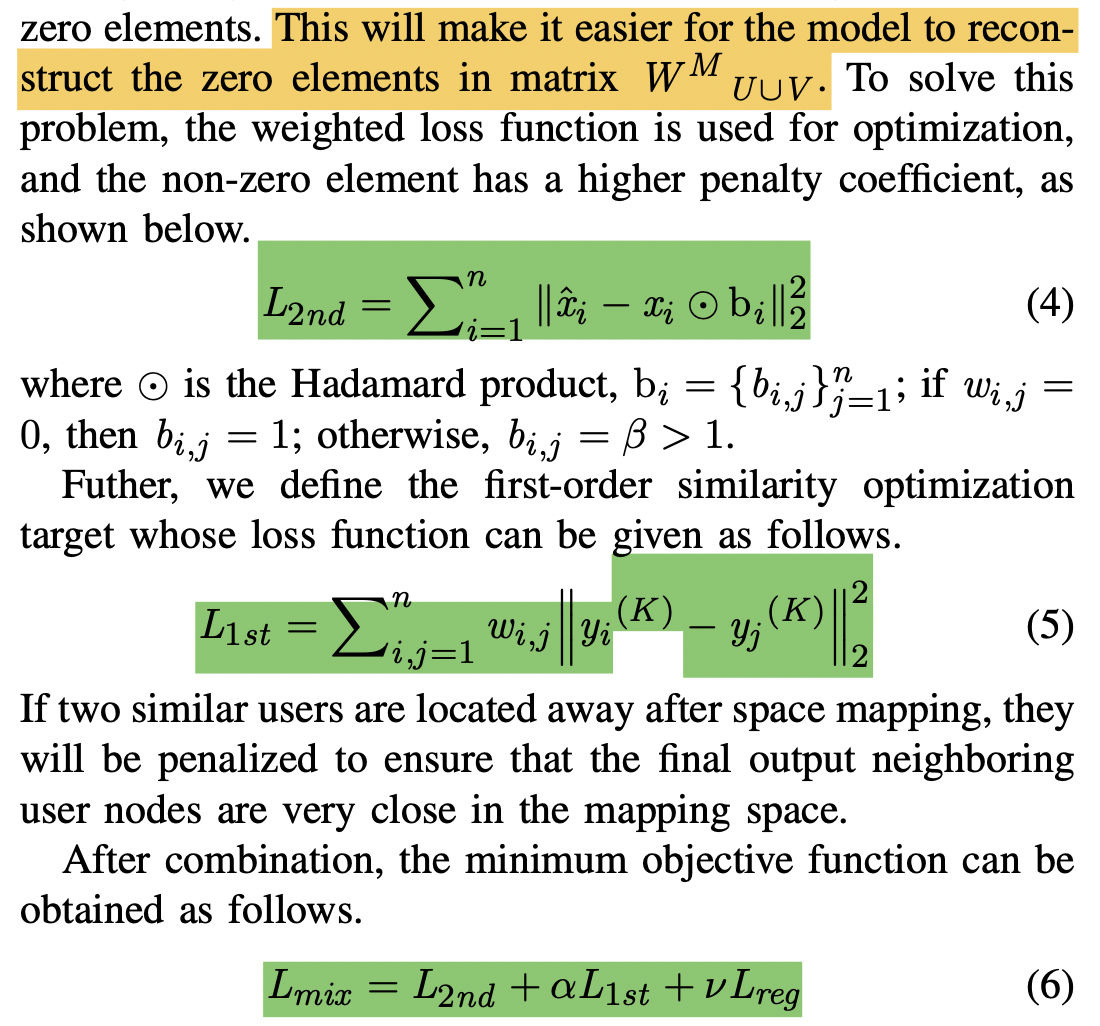
\includegraphics[width=0.6\linewidth]{Assets/SDNE.png}
\end{frame}

\begin{frame}{用户历史活动的表示}
	用户历史活动以一篇结构规范的文章来表示,我们希望从历史内容获得用户的社交兴趣(social interest)。
	\begin{itemize}
		\item 微博内容通常是是不太规范的汉语,关键词是最有价值的。
		\item 使用TF-IDF算法,计算每个用户的关键词权重。
	\end{itemize}
\end{frame}

\begin{frame}{用户在网络中影响力的量化方法(1)——内在/外在分类}
	用户的信息影响力分成内在影响和外在影响。我们回忆:\\
	用户属性 = 活跃度 + 表达方式偏好 + 社交影响力
	\begin{itemize}
		\item 内在影响指用户活跃度和转发倾向,这些是用户属性的一部分;论文注意到,用户活跃度越高,他/她参与内容转发的倾向性越大,论文更强调转发;
		\item 外在影响指用户对朋友和消息传播的影响力,这些也是用户属性的一部分。
	\end{itemize}
	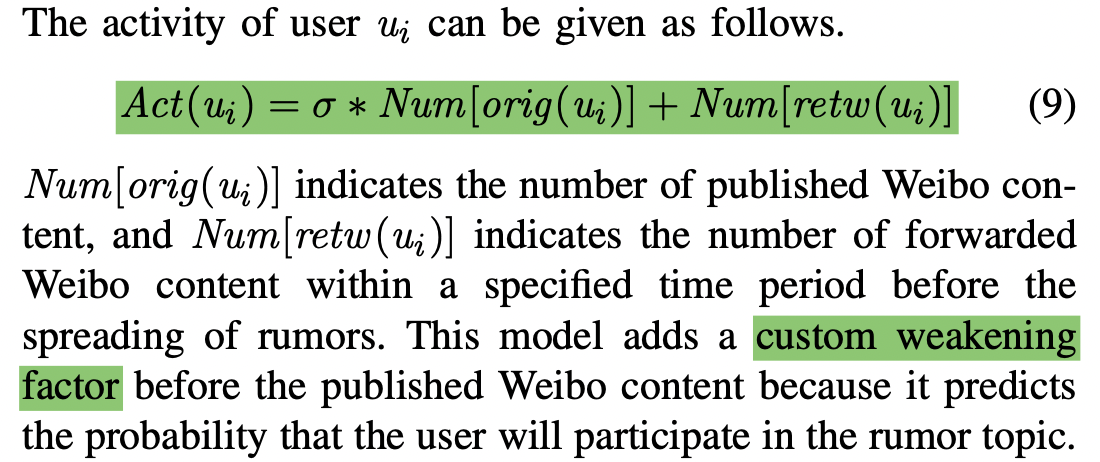
\includegraphics[width=0.6\linewidth]{Assets/Act.png}
\end{frame}

\begin{frame}{用户在网络中影响力的量化方法(2)——内在影响力}
	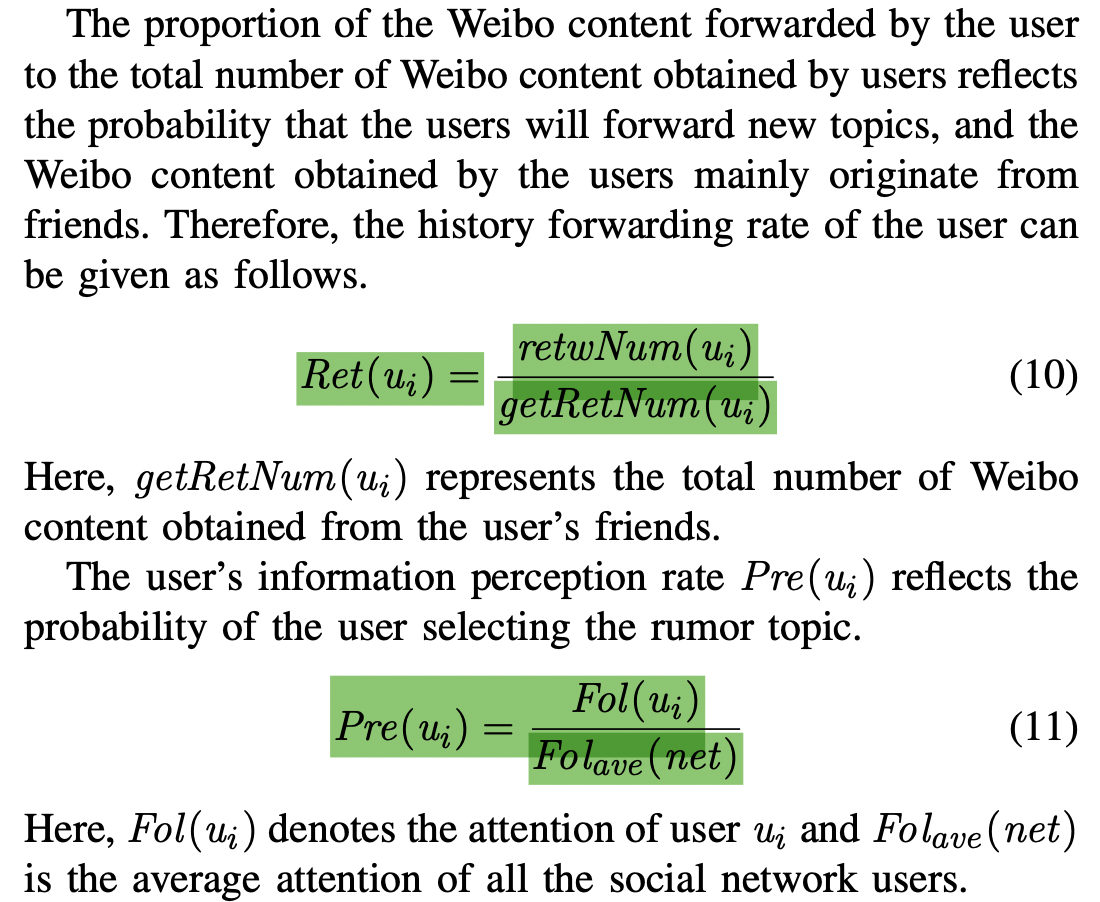
\includegraphics[width=0.8\linewidth]{Assets/内在影响.png}\\
	fin(ui) = Act(ui) × Ret (ui) × Pre (ui)\\
	用户内在影响力 = 活跃度 × 转发率 × 话题参与率
\end{frame}

\begin{frame}{用户在网络中影响力的量化方法(3)——外在影响力}
	我们讨论uj对ui的影响力:
	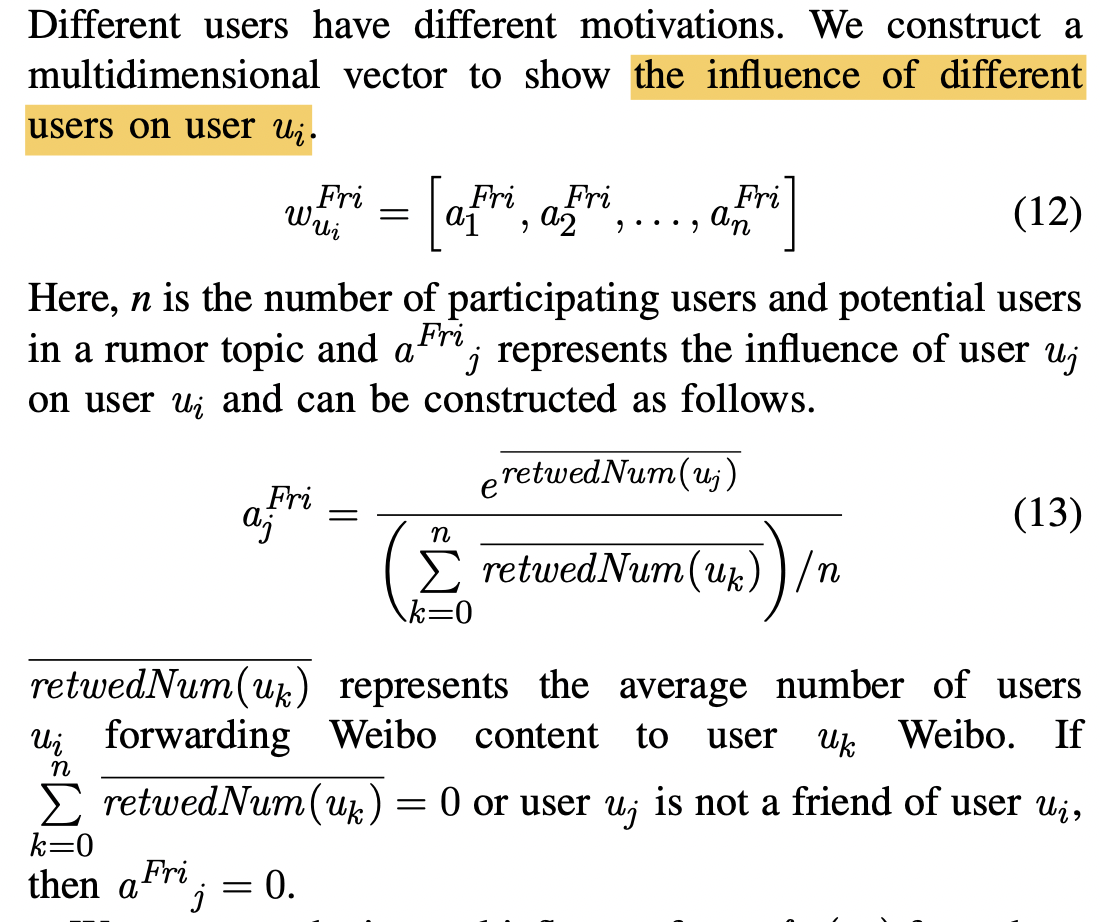
\includegraphics[width=0.6\linewidth]{Assets/外在影响.png}\\
	fout(ui, uj) = aFrij × Pop(t)\\
	用户j对i的外在影响力同时受两者之间转发率和内容流行度影响。
\end{frame}

\begin{frame}{用户j对i的影响——内在和外在,谣言和辟谣}
	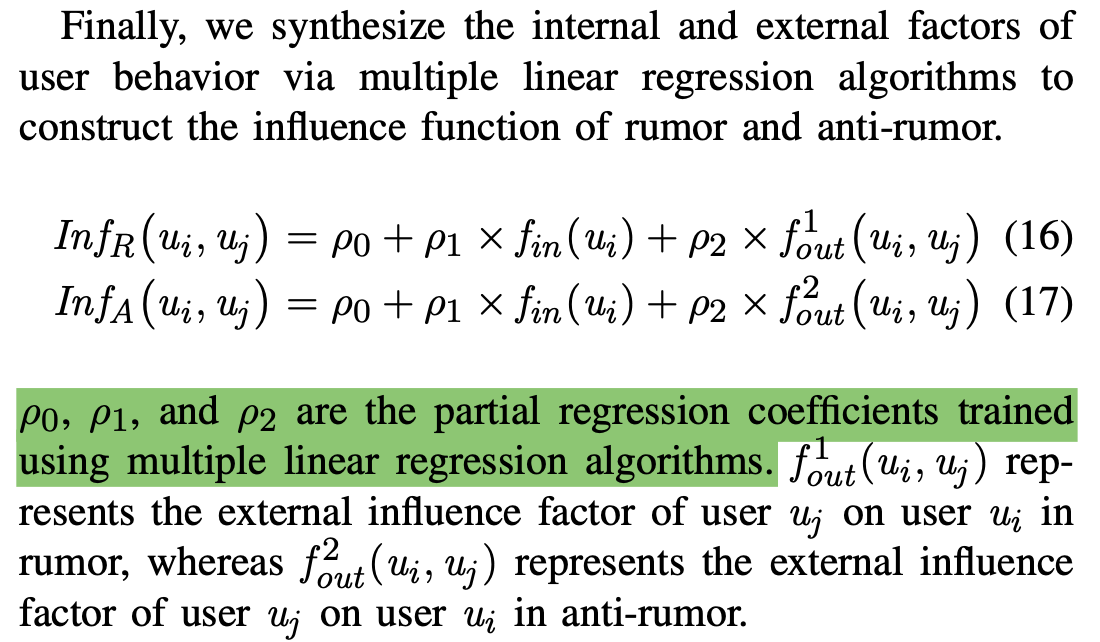
\includegraphics[width=0.8\linewidth]{Assets/Inf_RA.png}\\
	这里涉及了对3个系数的多元线性回归求解,论文作者并未孤立地考虑辟谣怎样抑制谣言,他从描述现实情况出发,尊重了谣言和辟谣并存的客观事实,优雅地统一了谣言和辟谣。两者从本质上是相通的,用户有内在倾向,它们也借助社交网络传播。
\end{frame}

\begin{frame}{进化博弈论模型构造(1)——博弈场景}
	用户的游戏策略有两种,即“转发谣言”和“转发辟谣信息”。设他的相邻用户组中转发谣言和转发辟谣信息的比例分别是P1和P2。论文未考虑那些惰性相邻用户,即 P1 + P2 = 1。我们容易构造利润函数,并给出uj对ui的“影响因子”:
	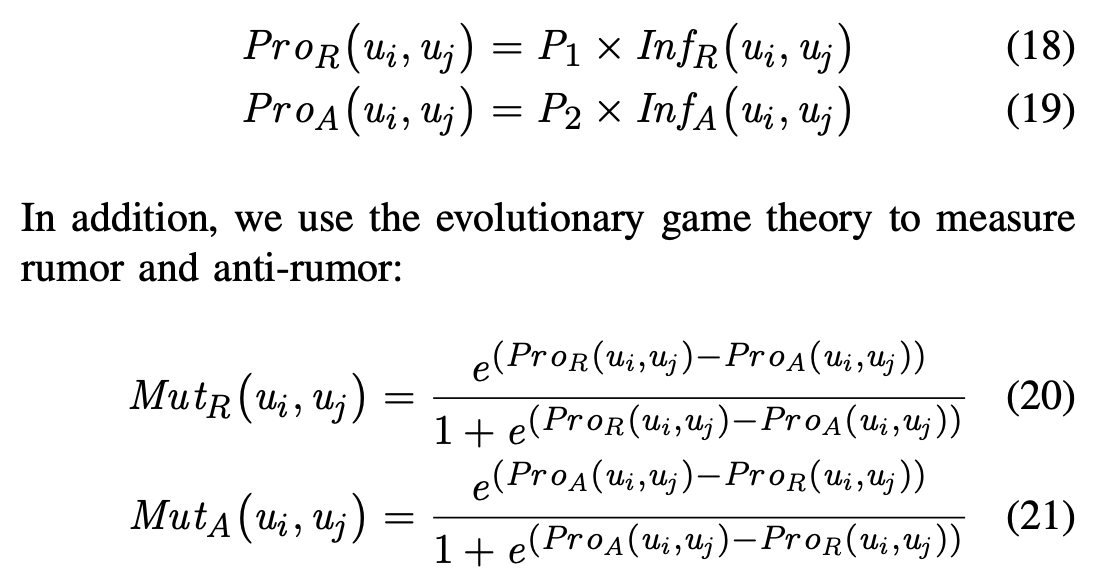
\includegraphics[width=0.8\linewidth]{Assets/进化博弈论-1.png}
\end{frame}

\begin{frame}{进化博弈论模型构造(2)——谣言和辟谣影响力矩阵}
	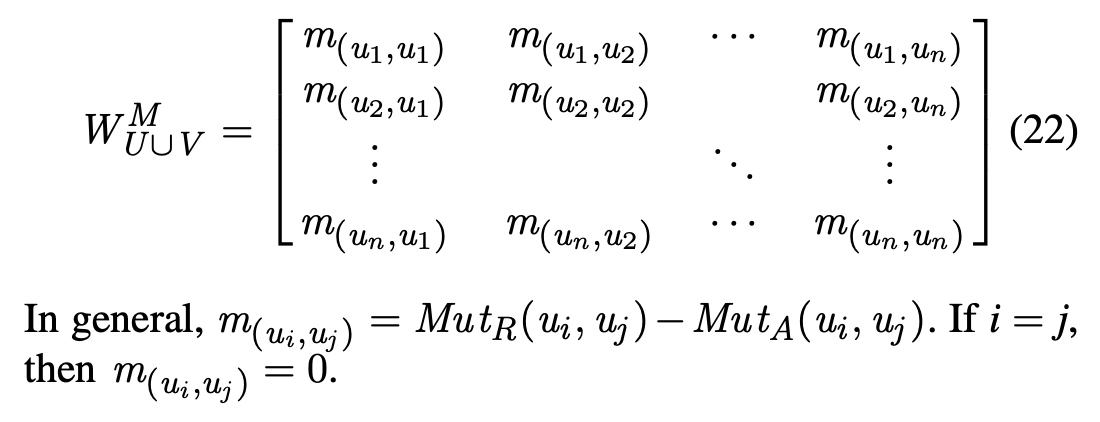
\includegraphics[width=0.8\linewidth]{Assets/进化博弈论-2.png}
\end{frame}

\begin{frame}{数据集划分和复杂度}
	通常,在深度学习模型训练中,我们选择80%的数据作为训练集,10%的数据作为测试集,以及10%的数据作为验证集。\\
	如果我们使用这种方法训练模型,则会发生模型过度拟合。我们根据标签选择了训练集,使谣言用户,反谣言用户和潜在用户的比例为1:1:2。在完成模型训练后,我们会应用另一个谣言主题作为模型的测试和验证集。\\
	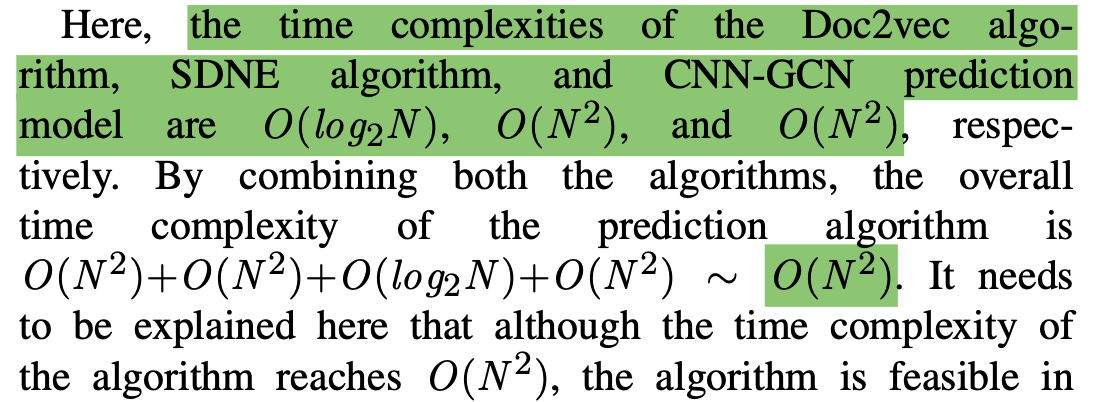
\includegraphics[width=0.8\linewidth]{Assets/时间复杂度.png}\\
	真实网络是稀疏的,另外,僵尸用户的存在是不可忽视的,这些导致实际时间复杂度更低。
\end{frame}

\begin{frame}{构造影响矩阵的伪代码}
	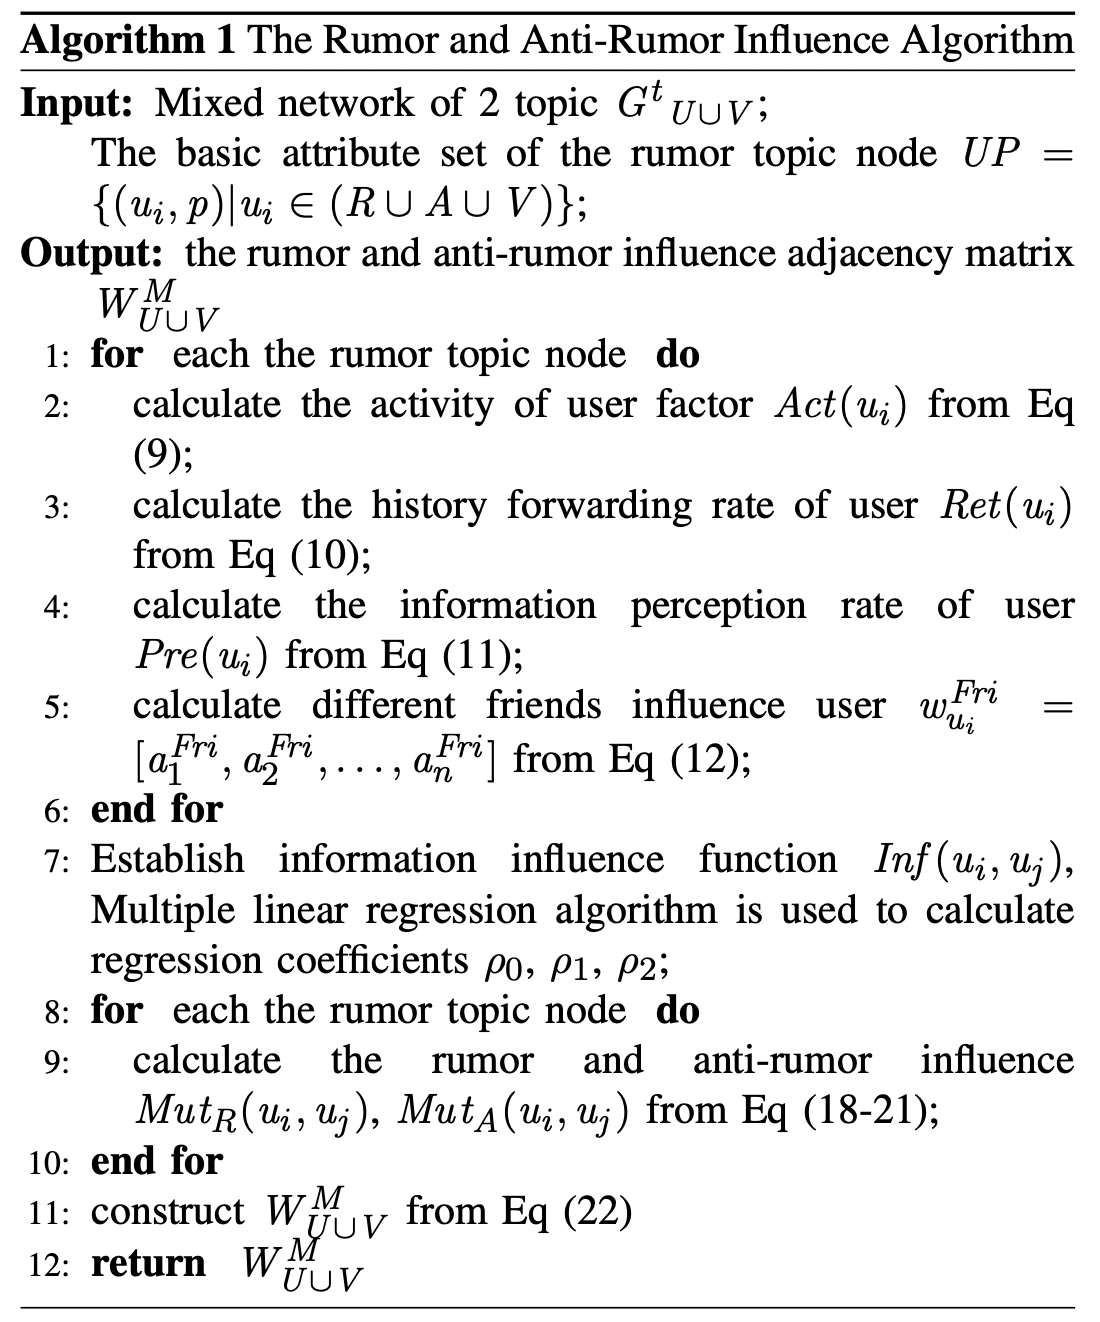
\includegraphics[width=0.6\linewidth]{Assets/算法1.png}
\end{frame}

\begin{frame}{用户行为算法的伪代码}
	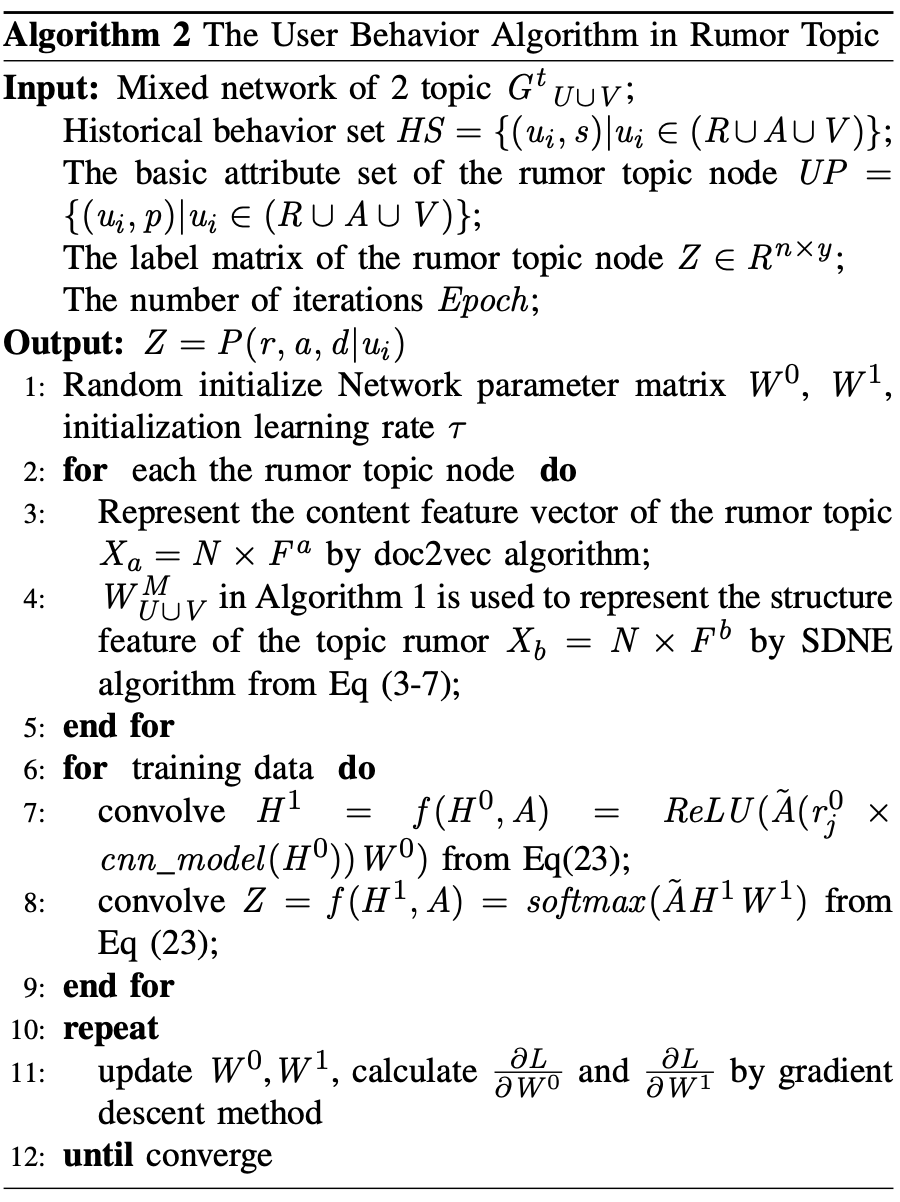
\includegraphics[width=0.6\linewidth]{Assets/算法2.png}
\end{frame}

\begin{frame}{实验配置}
	\begin{itemize}
		\item 数据集:新浪微博数据集,来自清华大学Aminer团队。
		\item 谣言主题:选择了4个产生了谣言的新闻主题——2011年甬台温铁路列车追尾事故(A)、韩寒被质疑造假事件(B)、湖南黄金大米事件(C)和悍匪周克华被击毙(D)。这些新闻事件均有谣言和辟谣信息共存。
		\item 事件C存在多轮谣言传播。
		\item 事件D中周克华未被击毙被及时辟谣。
	\end{itemize}
\end{frame}

\begin{frame}{新闻主题的谣言和辟谣信息数据规模}
	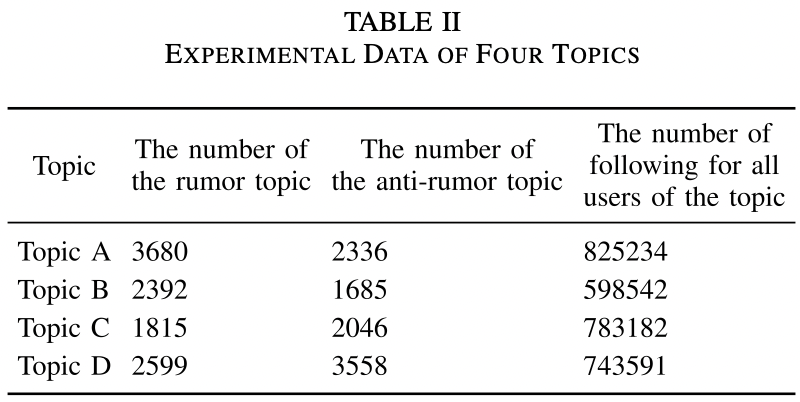
\includegraphics[width=\linewidth]{Assets/表2.png}
\end{frame}

\begin{frame}{新闻主题的谣言和辟谣信息参与者规模}
	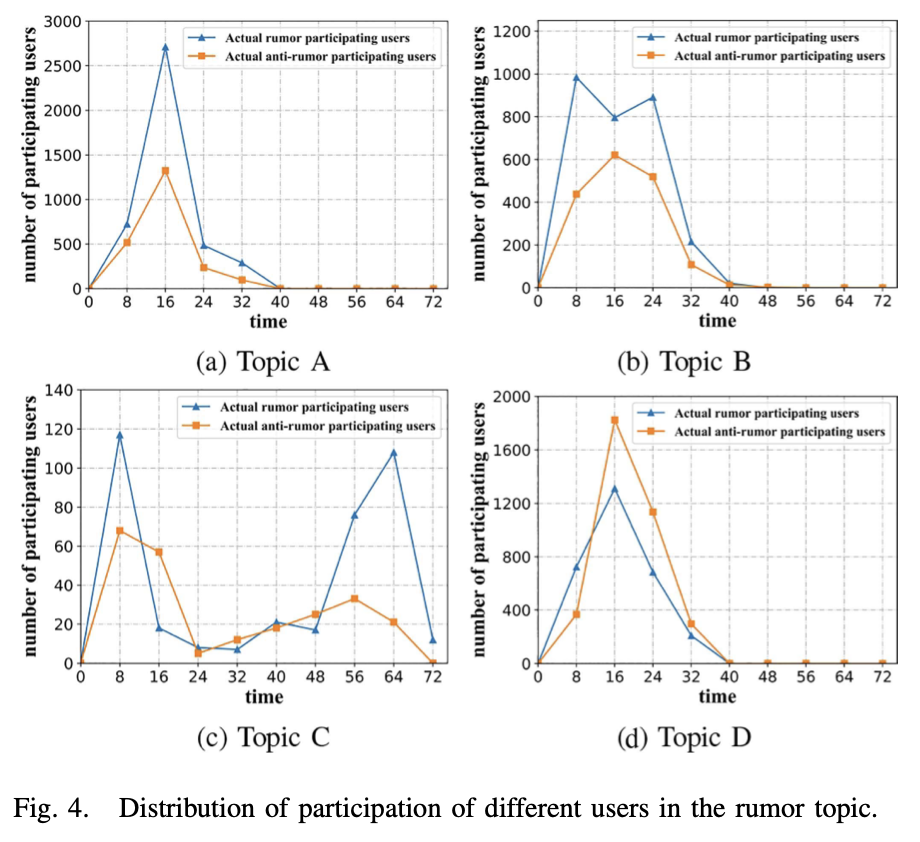
\includegraphics[width=0.8\linewidth]{Assets/图4.png}
\end{frame}

\begin{frame}{表现评估方法}
	\begin{itemize}
		\item 测试步骤:对CNN-GCN模型进行模型参数分析;分析和比较学习性能;分析谣言分类效果;将模型跟基线方法进行比较来评估预测模型的能力。
		\item 基线方法:SUA-ACNN、ODW-ELM、Cloud-RBFNN、RPMTD等。
		\item 测试指标:Loss、Macro-Average (Macro-F1) 和 Micro-Average (Micro-F1)。Loss体现了关于谣言话题的预测模型的准确性。它的值越小意味着模型越好。Macro-F1和Micro-F1使用各自的混淆矩阵,使用不同的分类数据来计算F1分数。
	\end{itemize}
\end{frame}

\begin{frame}{对CNN-GCN模型进行模型参数分析(1)——GCN}
	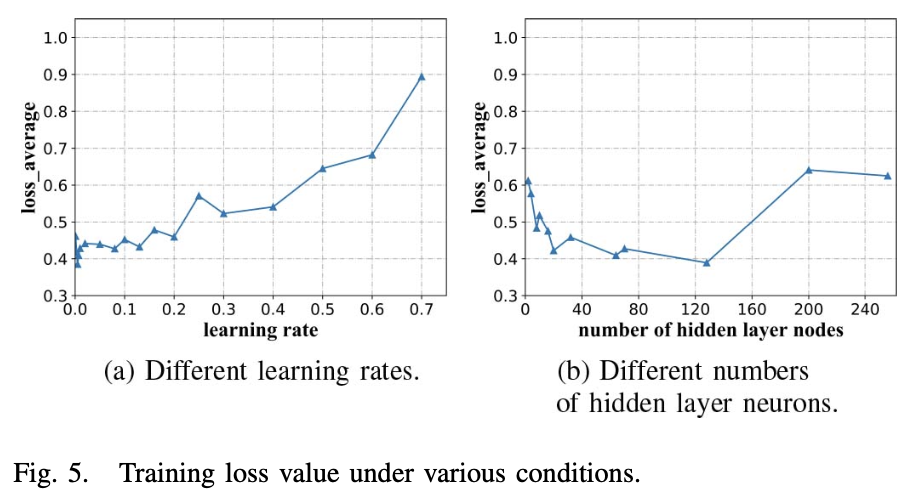
\includegraphics[width=0.8\linewidth]{Assets/图5.png}\\
	GCN:学习速率为0.05;隐藏层节点的数量为128。
\end{frame}

\begin{frame}{对CNN-GCN模型进行模型参数分析(2)——CNN}
	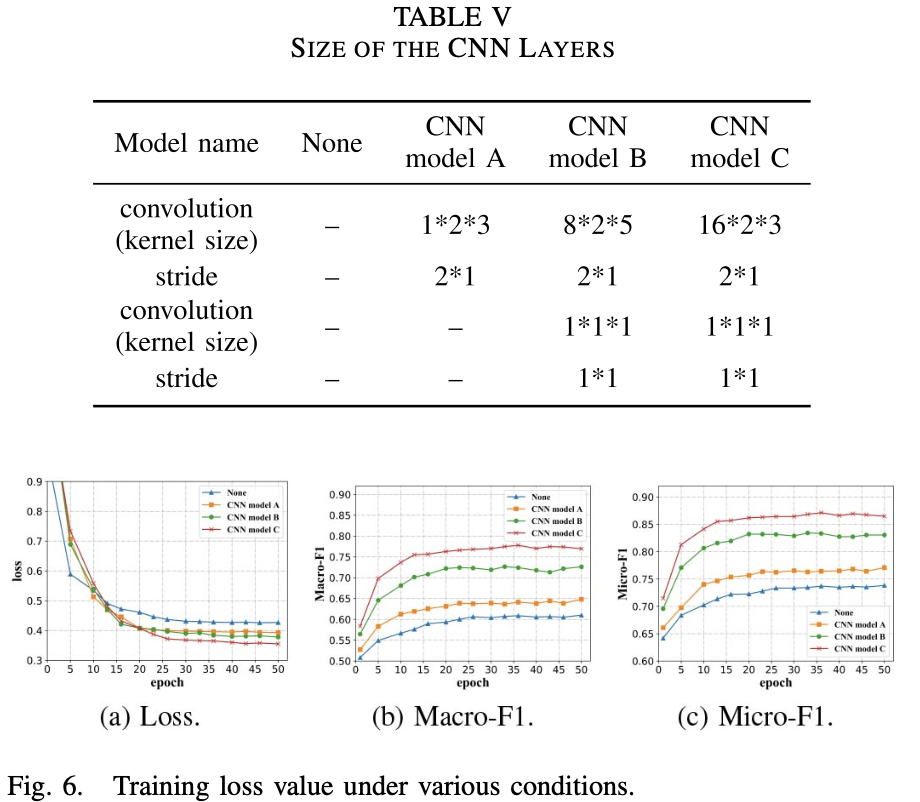
\includegraphics[width=0.8\linewidth]{Assets/表5_图6.png}\\
	选择了模型C。
\end{frame}

\begin{frame}{分析和比较学习性能——关键词提取和特征构建}
	特征组合:(1) SDNE, (2) Line, (3) Doc2vec, and (4) GolVe
	Group A:(1) + (3); Group B:(1) + (4); Group C:(2) + (3); and Group D:(2) + (4)\\
	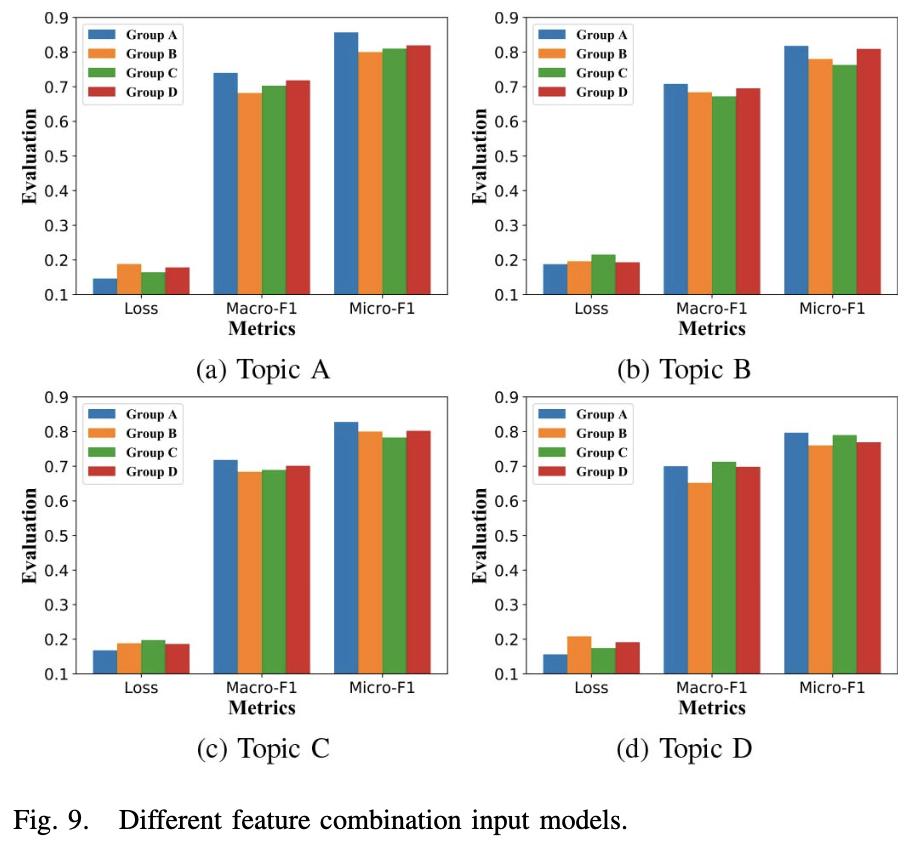
\includegraphics[width=0.6\linewidth]{Assets/图9.png}\\
	选择了Group A。
\end{frame}

\begin{frame}{分析谣言分类效果(1)——输入矩阵}
	\begin{itemize}
		\item 针对潜在用户,输入基于进化博弈论的影响矩阵会在较小程度上改善预测效果;
		\item 针对造/传谣和辟谣用户,输入基于进化博弈论的影响矩阵会显著改善预测效果。
	\end{itemize}
	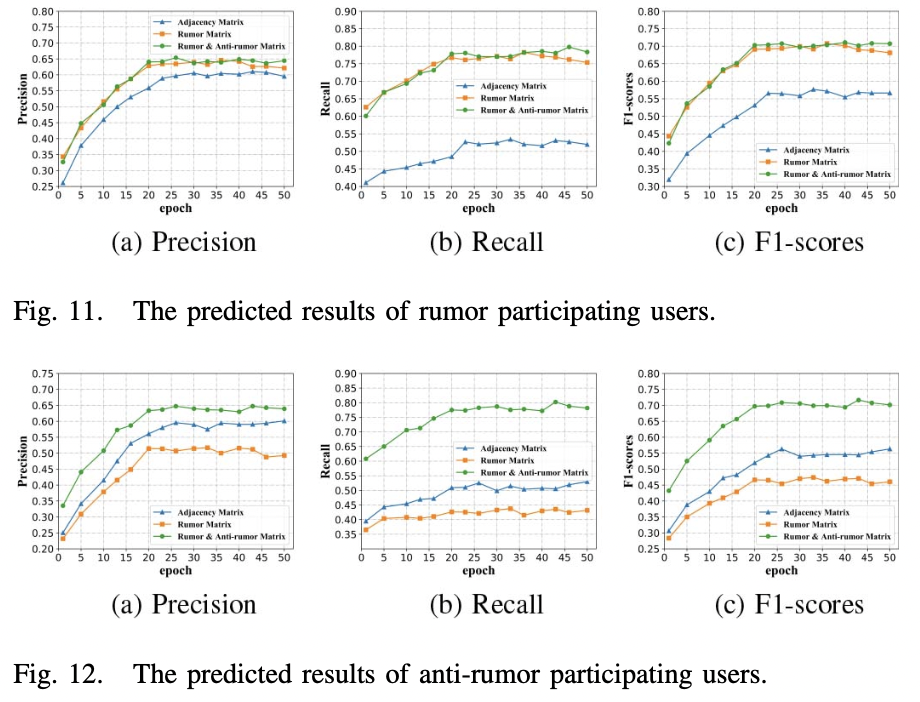
\includegraphics[width=0.6\linewidth]{Assets/图11_图12.png}
\end{frame}

\begin{frame}{分析谣言分类效果(2)——模型}
	CNN-GCN是最好模型。\\
	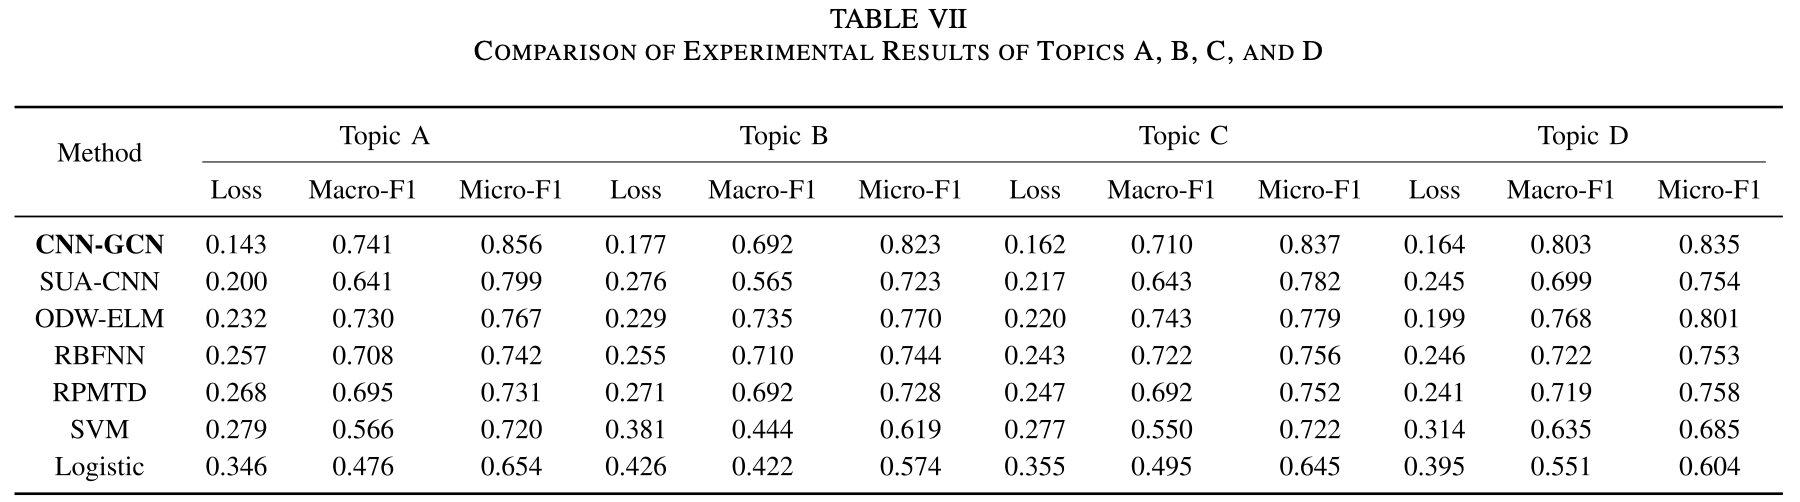
\includegraphics[width=\linewidth]{Assets/表7.png}
\end{frame}

\begin{frame}{将模型跟基线方法进行比较来评估预测模型的能力}
	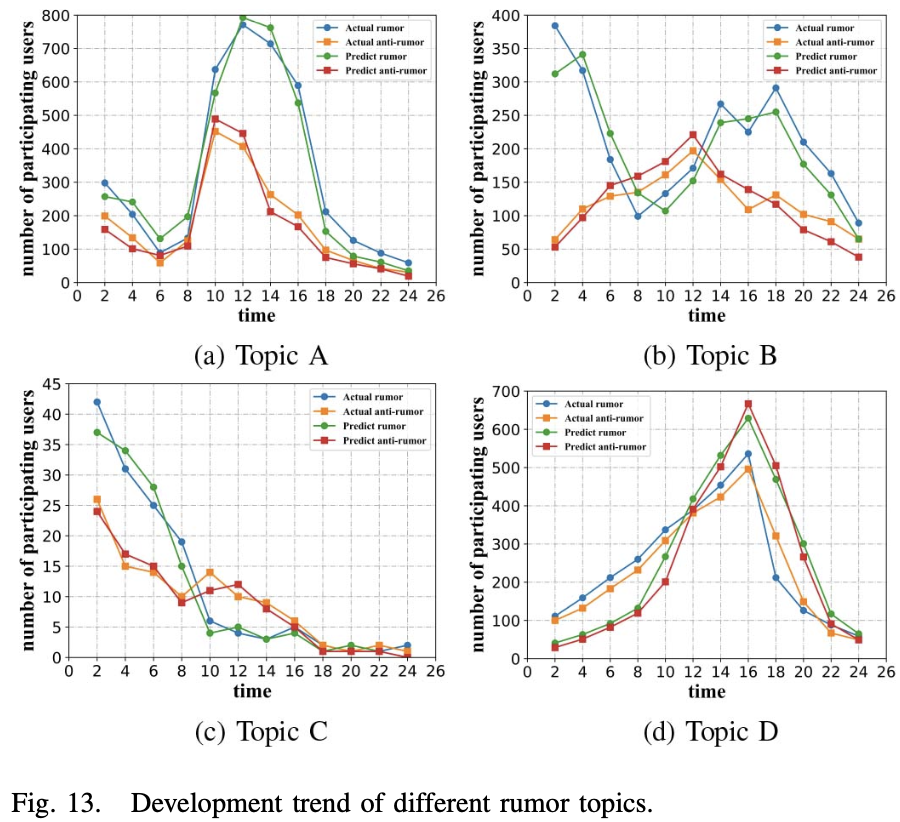
\includegraphics[width=0.8\linewidth]{Assets/图13.png}
\end{frame}

\begin{frame}{本文亮点}
	\begin{itemize}
		\item 内容饱满,预测效果好。本文有效地描述了谣言的发展趋势,根本在于良好地预测了用户在谣言网络中的角色变化。
		\item 本文成功地运用了博弈论,摒弃了辟谣对谣言单方面的遏制这样的思维。两者存在对抗的同时,也存在共生,作者优雅和精彩地描述了客观现实。
		\item 数据具有较强的说服力,在模型选择过程中进行了广泛比较和选择。
	\end{itemize}
\end{frame}

\begin{frame}
	谢谢!
\end{frame}

\end{document}
